\chapter{Preliminaries}\label{preliminaries}
In this chapter we have briefly described the necessary topics we need to
know before we go into Motifs. We have started with the most fundamental
part of life cells. Then from the cells, we have gone deeper into the genetic
materials the genes, DNA, RNA and Proteins. We have discussed about the flow
of information from the DNA to the Protein in detailed steps. We have illustrated the motif finding problem and classify different types of motifs. Later, we have shown building the consensus string from the alignment matrix and profile matrix. We have also discussed a consensus string evaluating function. We have concluded this chapter by giving a very simple brute-force motif finding algorithm.

\section{What is Life Made of}
In 1665 Robert Hooke discovered that every organisms
in living bodies are composed of individual compartments
known as cells\index{Cell}. With this huge discovery in
the field of Biology the study of life became the study of cells.

\subsection{Cells}
A cell is the smallest structural unit of an organism that
is capable of independent functioning. Moreover, a cell as a complex mechanical system with many moving parts which not only stores all the necessary information to make a
complete replica of itself but also contains all the machinery required to collect
and manufacture its components, carry out the copying process, and start its new offspring. So, cells are the fundamental working units of every living system.

\subsection{Life Cycle of a Cell}
A great diversity of cells exist in nature, but they all have some common
features. All cells have a life cycle: they are born, eat, replicate, and die
illustrated in \Cref{fig:cellcycle}

\begin{figure}[!tb]
	\centering
	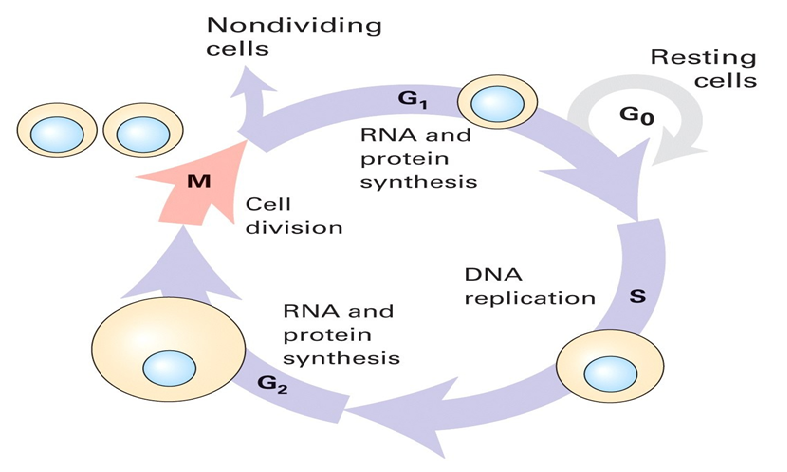
\includegraphics[width=0.8\textwidth]{figures/cellcycle}
	\caption{Life cycle of a cell.}
	\label{fig:cellcycle}
\end{figure}

\subsection{Types of Cells}
We can differentiate cells into two types based on their
structures. They are called \textit{Prokaryotic} and \textit{Eukaryotic} cells.
Prokaryotic\index{Cell!Prokaryotic} cells do not contain a nucleus or any other membrane-bound organelle.
Only contain one piece of circular DNA and no mRNA post transactional modification.
Bacteria are an example of prokaryotes.
Eukaryotic\index{Cell!Eukaryotic} cells contain membrane-bound organelles, including a nucleus. 
They contain multiple chromosomes. Eukaryotes can be single-celled or multi-celled such as humans, plants and fungi.

\begin{figure}[H]
	\centering
	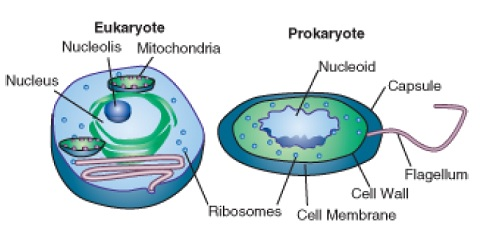
\includegraphics[width=0.7\textwidth]{figures/celltype}
	\caption{Prokaryotic and Eukaryotic cells.}
	\label{fig:celltype}
\end{figure}

\section{Genetic Material of Life}
All the genetic materials of a organism is called Genome\index{Genome}.
The genome is an organism’s complete set of DNA, including all of its genes. 
Each genome contains all of the information needed to build and maintain that organism.
They includes both the genes and non-coding sequences of the DNA.
A bacteria genome contains about 600,000 DNA base pairs while
human and mouse genomes have some 3 billion. Different organisms have different numbers of chromosomes, suggesting that they might carry information specific for each species. Human genome has 46 (23 pairs) distinct chromosomes. Each chromosome contains many genes. 


\subsection{Genes}
Genes\index{Gene} are discrete units of hereditary information located on the chromosomes and consisting of DNA. Gregor Mendel's experiments with garden peas suggested the existence of genes that were responsible for inheritance. Genes are small sections of DNA within the genome that code for proteins. They contain the instructions for our individual characteristics- like eye and hair color. 
The human genome contains approximately 25000 protein-coding genes.
So, we can say that the main job of genes-
\begin{itemize}
	\item Storing information about the characteristics. 
	\item They express the genotype and phenotypes.
	\item The main task of genes is to produce proteins.
	\item Each gene contains the information required to build specific proteins needed in an organism.
\end{itemize}
 
\subsection{DNA}
DNA\index{DNA} or deoxyribonucleic acid, is the hereditary material in humans and almost all other organisms. Nearly every cell in a person’s body has the same DNA. DNA was discovered by Johann Friedrich Miescher by isolating a substance he called \textit{nuclein} from the nuclei of white blood cells. The information in DNA is stored as a code made up of four chemical bases: \textit{Adenine} (A), \textit{Guanine} (G), \textit{Cytosine} (C), and \textit{Thymine} (T). Human DNA consists of about 3 billion bases, and more than 99 percent of those bases are the same in all people.

DNA bases pair up with each other, A with T and C with G, to form units called base pairs. Each base is also attached to a sugar molecule and a phosphate molecule. Together, a base, sugar, and phosphate are called a nucleotide. Nucleotides are arranged in two long strands that form a spiral called a double helix. The structure of the double helix is somewhat like a ladder, with the base pairs forming the ladder's rungs and the sugar and phosphate molecules forming the vertical sidepieces of the ladder.

\begin{figure}[!tb]
	\centering
	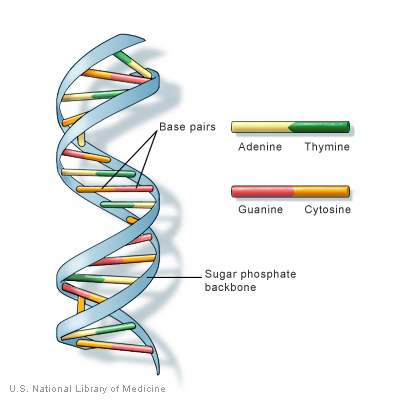
\includegraphics[width=0.7\textwidth]{figures/dna}
	\caption{DNA double helix formed by base pairs attached to a sugar-phosphate backbone.}
	\label{fig:dna}
\end{figure}


Although,DNA has a double helix structure, it is not symmetric. It has a ``forward" and ``backward" direction.  The ends are labeled 5' and 3' after the Carbon atoms in the sugar component like 5' AATCGCAAT 3'. DNA always reads 5' to 3' for transcription replication. DNA is a polymer of Sugar-Phosphate-Base. Bases held together by \textit{Hydrogen} bonding to the opposite strand. Base pairs of G and C contain three hydrogen bonds and base pairs of A and T contain two hydrogen bonds. As a reason, G-C base-pairs are more stable than A-T base pairs. 

\begin{figure}[!tb]
	\centering
	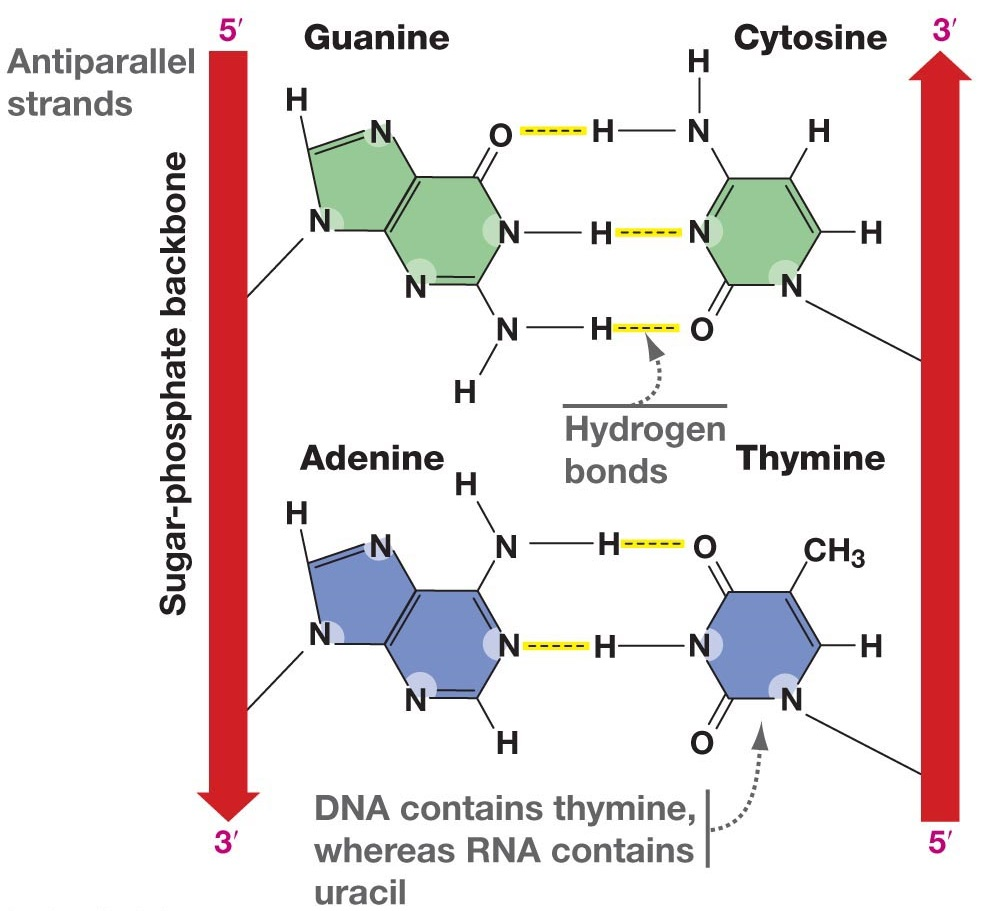
\includegraphics[width=0.7\textwidth]{figures/dna2}
	\caption{Hydrogen bonds between A-T and C-G.}
	\label{fig:dna2}
\end{figure}


\subsection{RNA}
RNA\index{RNA} or ribonucleic acid, is similar to DNA chemically. It usually has only a single strand. RNA contains ribose while DNA contains deoxyribose. Deoxyribose lacks one oxygen atom. RNA contains the bases \textit{Adenine} (A), \textit{Uracil} (U) instead of \textit{Thymine} in DNA, \textit{Cytosine} (C) and \textit{Guanine} (G).
Unlike DNA, RNA comes in a variety of shapes and types. While DNA contains double helix, RNA may be of more than one type. RNA is usually single-stranded, while DNA is usually double-stranded. Some forms of RNA can form secondary structures by pairing up with itself. This can have change it's properties. DNA and RNA can also pair with each other. RNA molecules are involved in protein synthesis and sometimes in the transmission of genetic information.

\begin{figure}[!tb]
	\centering
	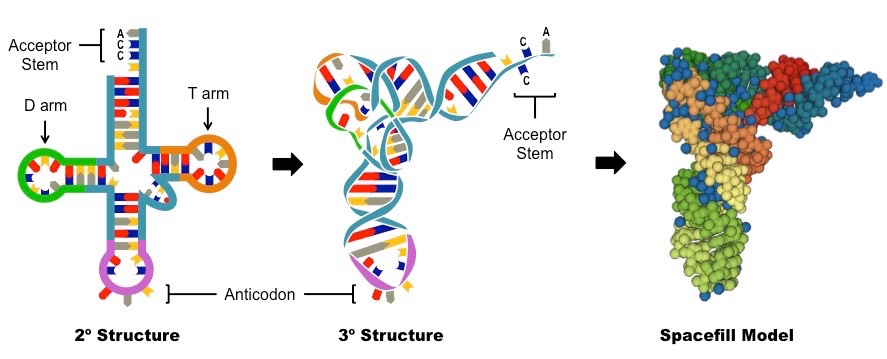
\includegraphics[width=0.9\textwidth]{figures/trna}
	\caption{tRNA linear and comples structure.}
	\label{fig:rna}
\end{figure}

Several types of RNA exists. They can be classified by various functions like:
\begin{itemize}
	\item \textbf{mRNA - Messenger RNA :} Encodes amino acid sequence of a polypeptide. When a Bioinformatician says ``RNA" it usually means mRNA.
	\item \textbf{tRNA - Transfer RNA :} Brings amino acids to ribosomes during translation.
	\item \textbf{rRNA - Ribosomal RNA :} With ribosomal proteins, makes up the ribosomes, the organelles that translate the mRNA.
\end{itemize}

\subsection{Protein}
Protein\index{Protein} is a highly complex substance that is present in all living organisms. They are responsible for most of the complex functions that make life possible. They are polymer of smaller subunits called amino acids. Also called ``poly-peptides". There are twenty amino acids, each coded by three-base-sequences in DNA called ``codons" whish are degenerate. Different chemical properties cause the protein chains to fold up into specific three-dimensional structures that define their particular functions in the cell. 

\begin{figure}[!tb]
	\centering
	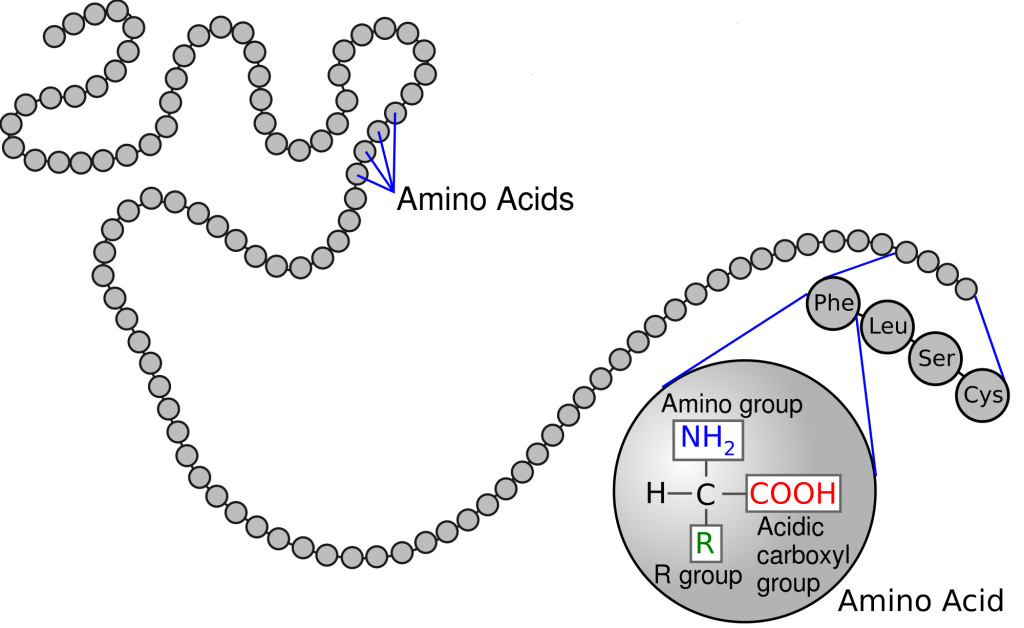
\includegraphics[width=0.8\textwidth]{figures/protein}
	\caption{Primary protein structure - chain of amino acids.}
	\label{fig:protein}
\end{figure}

Proteins do all essential work for the cell like:
\begin{itemize}
	\item Build cellular structures.
	\item Digest nutrients.
	\item Execute metabolic functions.
	\item Mediate information flow within a cell and among cellular communities. 
\end{itemize}

\subsection{Mutation}
Mutation\index{Mutation} is the permanent alteration of the nucleotide sequence of the genome of an organism or DNA or other genetic elements. Mutations result from errors during DNA replication or other types of damage to DNA, which then may undergo error-prone repair or cause an error during other forms of repair or else may cause an error during replication. Mutations can serve the organism in three ways:
\begin{itemize}
	\item The Good : A mutation can cause a trait that enhances the organism’s function. For example mutation in the sickle cell gene provides resistance to malaria.
	\item The Bad : A mutation can cause a trait that is harmful, sometimes fatal to the organism. For example Huntington’s disease, a symptom of a gene mutation is a degenerative disease of the nervous system.
	\item The Silent : A mutation can simply cause no difference in the function of the organism.
\end{itemize}


\section{What Carries Information Between DNA to Proteins}
The information for making proteins is stored in DNA. There is a process (transcription and translation) by which DNA is converted to protein. By understanding this process and how it is regulated we can make predictions and models of cells.

\subsection{Central Dogma of Molecular Biology}\index{Central Dogma}
The paradigm that DNA directs its transcription to RNA, which is then translated into a protein is called central dogma of molecular biology\index{Central Dogma of Molecular Biology}. It was first proposed by Francis Crick. The central dogma of molecular biology explains the flow of genetic information, from DNA to RNA, to make a functional product, a protein.

The central dogma states that the pattern of information that occurs most frequently in our cells is:
\begin{itemize}
	\item From existing DNA to make new DNA (DNA replication).
	\item From DNA to make new RNA (transcription).
	\item From RNA to make new proteins (translation).
\end{itemize}

\begin{figure}[!tb]
	\centering
	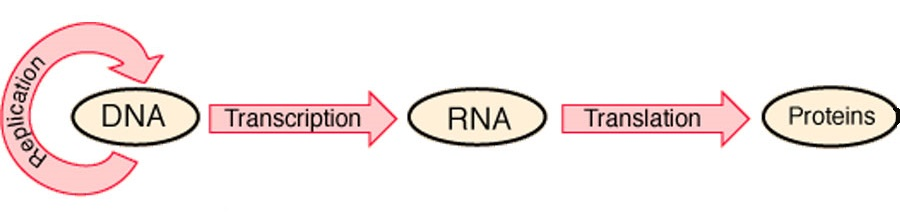
\includegraphics[width=0.9\textwidth]{figures/dogma}
	\caption{Central dogma of molecular biology.}
	\label{fig:dogma}
\end{figure}

\subsection{DNA$\,\to\,$RNA: Transcription}
Transcription\index{Transcription} is the process by which DNA is copied to mRNA, which carries the information needed for protein synthesis. Transcription takes place in two broad steps. First, pre-messenger RNA is formed, with the involvement of RNA polymerase enzymes. The process relies on Watson-Crick base pairing, and the resultant single strand of RNA is the reverse-complement of the original DNA sequence. The pre-messenger RNA is then edited to produce the desired mRNA molecule in a process called RNA splicing.

\subsubsection{Formation of pre-messenger RNA}
The mechanism of transcription has parallels in that of DNA replication. As with DNA replication, partial unwinding of the double helix must occur before transcription can take place, and it is the RNA polymerase enzymes that catalyze this process. Unlike DNA replication, in which both strands are copied, only one strand is transcribed. The strand that contains the gene is called the sense strand, while the complementary strand is the antisense strand. The mRNA produced in transcription is a copy of the sense strand, but it is the antisense strand that is transcribed. 

Ribonucleotide triphosphates (NTPs) align along the antisense DNA strand, with Watson-Crick base pairing (A pairs with U). RNA polymerase joins the ribonucleotides together to form a pre-messenger RNA molecule that is complementary to a region of the antisense DNA strand. Transcription ends when the RNA polymerase enzyme reaches a triplet of bases that is read as a ``stop" signal. The DNA molecule re-winds to re-form the double helix. The \Cref{fig:transcription} illustrates the process.
\begin{figure}[!tb]
	\centering
	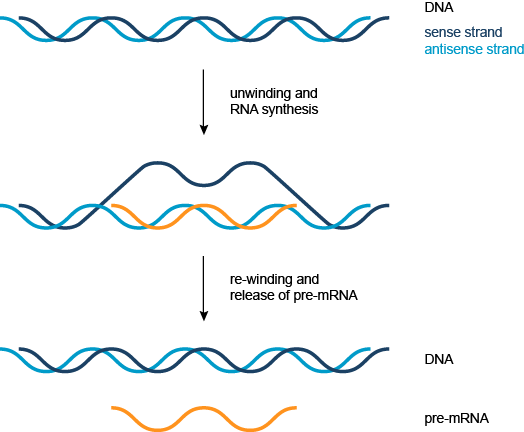
\includegraphics[width=0.8\textwidth]{figures/transcription}
	\caption{Formation of pre-messenger RNA.}
	\label{fig:transcription}
\end{figure}

\subsubsection{Splicing}\index{Splicing}
In Eukaryotic cells, RNA is processed between transcription and translation. Unprocessed RNA is composed of \textit{Introns} and \textit{Extrons}. The pre-mRNA is chopped up to remove the introns and create mRNA in a process called RNA splicing. Sometimes alternate RNA processing can lead to an alternate protein as a result. 
\begin{figure}[!tb]
	\centering
	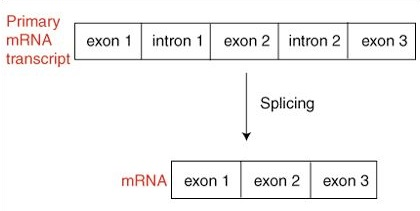
\includegraphics[width=0.6\textwidth]{figures/splicing}
	\caption{RNA splicing: Introns are spliced from the pre-mRNA to give mRNA.}
	\label{fig:splicing}
\end{figure}

\subsection{RNA$\,\to\,$Protein: Translation}\index{Translation}
There are twenty types of tRNAs, and twenty types of amino acids.
Each type of amino acid binds to a different tRNA, and the tRNA molecules
have a three-base segment called an anticodon that is complementary to the
``codon" in the mRNA. As in DNA base-pairing, the anticodon on the tRNA
sticks to the codon on the RNA, which makes the amino acid available to the
ribosome to add to the polypeptide chain. When one amino acid has been
added, the ribosome shifts one codon to the right, and the process repeats.
The process of turning an mRNA into a protein is called translation, since it
translates information from the RNA into the protein. 

\begin{figure}[!tb]
	\centering
	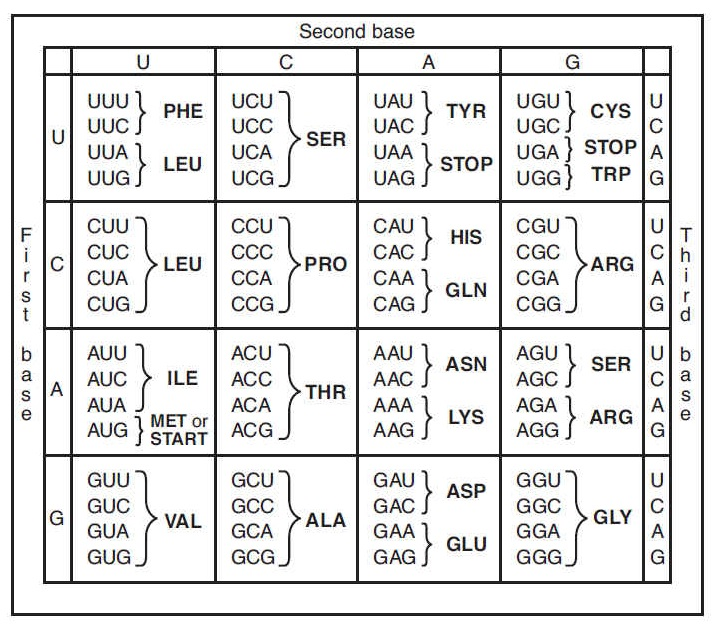
\includegraphics[width=0.6\textwidth]{figures/codon}
	\caption{The genetic code, from the perspective of mRNA.}
	\label{fig:codon}
\end{figure}


%%%%%has to modify
\section{Motifs in Details}
Motif\index{Motif} usually means a pattern. For any sequence
of objects to be called a pattern, it has to have at least
more than one instance. To define more precisely, a motif
should have significantly higher occurrence in a given array
or list compared to what you would obtain in a randomized
array of same components. Here array means an arranged set
such as a genome or a protein structure. Genome is an array
of nucleotides and protein structure is an array of amino acids.

\subsection{Sequence Motifs}
By sequence motif\index{Motif!Sequence Motif} we mean a pattern
of nucleotide or amino acid that has specific biological
significance. In other words, they are pattern of a DNA array or
protein sequence. They may be also called regulatory sequence
motifs. This kind of motifs are commonly studied in bioinformatics.
They are becoming increasingly important in the analysis of gene
regulation. In our thesis we will only discuss about this type of motifs.

\subsection{Structural Motifs}
Structural motifs\index{Motif!Structural Motif} are a super-secondary
structure in a chain like biological molecules such as protein.
It is formed by three dimensional alignment of amino acids
which may not be adjacent.

\subsection{Regulatory Motifs in DNA}
Regulatory motifs\index{Regulatory Motifs} are some short nucleotide
sequence that regulates the expression of genes such as controlling
the situations under which the genes will be turned on or off.
For example:~\cite{jones2004introduction} Fruit flies have a small
set of \textit{immunity genes} that are dormant
in their genome. But when its organisms get infected somehow the genes
got switched on. It turns out that many immunity genes in
the fruit fly genome have strings that are reminiscent of TCGGGGATTTCC,
located upstream of the genes start. This string are called $ _{NF-\kappa}$B
binding sites which are important examples of regulatory motifs. Proteins
known as \textit{transcription factors} bind to these motifs, encouraging
RNA polymerase to transcribe the downstream genes.

\subsection{Regulatory Regions}
As discussed in~\cite{Riethoven2010} regulation of gene expression
is an essential part of every organism. Certain regions,
called cis-regulatory elements, on the DNA are footprints for
the trans-acting proteins involved in transcription. DNA
regions involved in transcription and transcriptional regulation
are called regulatory regions (RR).\index{Regulatory Motifs!Regulatory Regions}
Every gene contains a RR typically
stretching 100-1000 bp upstream of the transcriptional start site.
In  \Cref{fig:rr} we see the structure of a eukaryotic protein coding gene. 
Regulatory sequence controls when and where expression
occurs for the protein coding region (red). Promoter and enhancer
regions (yellow) regulate the transcription of the gene into a
pre-mRNA which is modified to remove introns (light grey) and
add a 5' cap and ploy-A tail (dark grey). The mRNA 5' and 3'
untranslated regions (blue) regulate translation into the
final protein product.


\begin{figure}[!tb]
	\centering
	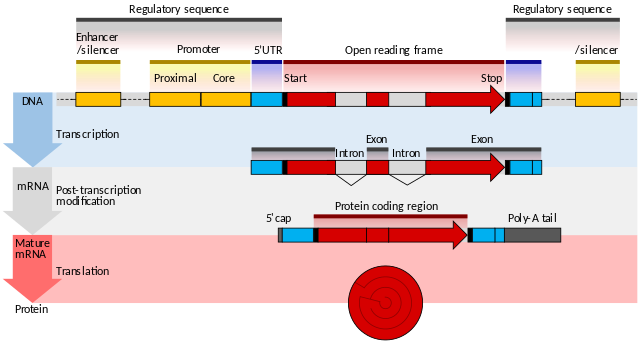
\includegraphics[width=0.9\textwidth]{figures/rr}
	\caption{The structure of a eukaryotic protein-coding gene.}
	\label{fig:rr}
\end{figure}


\subsection{Transcription Factor Binding Sites}
\index{Regulatory Motifs!Transcription Factor Binding Sites}
A transcription factor (TF) is a protein that can bind to DNA
and regulate gene expression. The region of the gene to which
TF binds is called a transcription factor binding site (TFBS).
TFs influence gene expression by binding to a specific location
in the respective gene’s regulatory region which is known as
TFBSs or motifs.~\cite{wei2007comparative} TFBS can be located
anywhere within the RR. TFBS may vary slightly across different
regulatory regions since non-essential bases could mutate.
TFBSs are a part of either the promoter or enhancer region of a gene.
A promoter sits upstream and contains three important regions-
the regulatory protein binding site, the transcription factor
binding site, and the RNA polymerase binding site.
In \Cref{fig:tfbs} we see a picture of promoter
and enhancer. An enhancer is usually far upstream of a gene.

\begin{figure}[!tb]
	\centering
	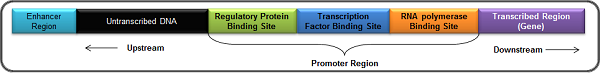
\includegraphics[width=0.9\textwidth]{figures/tfbs}
	\caption{Transcription Factor Binding Sites.}
	\label{fig:tfbs}
\end{figure}

\section{To The Motif Finding Problem}\index{Motif Finding Problem}
Our target is to identify a motif from a DNA sequence. In our study
we only deal with transcription factor binding sites. We will give
the formal definition of the motif finding problem later. Assume
that we are given some DNA sequence of nucleotides which are generated
randomly. Now, we want to find a secret pattern that occurs at least
one time in every given DNA sequence without any prior knowledge
about how it looks like. This pattern is our motif.

Some complications encountered while finding motifs:
\begin{itemize}
	\item We do not know the motif sequence.
	\item Hence we donot know what to search for in the DNA sequence.
	\item We do not know where the motifs are located relative to
	the starting index of the sequence.
	\item Motifs can differ in one or more positions in their
	sequence which is called mutations.
	\item How to discern functional motifs from random ones?
	
\end{itemize}

The idea is illustrated in the \Cref{fig:seq1}, \Cref{fig:seq2}
and \Cref{fig:seq2}.

\begin{figure}[H]
	\centering
	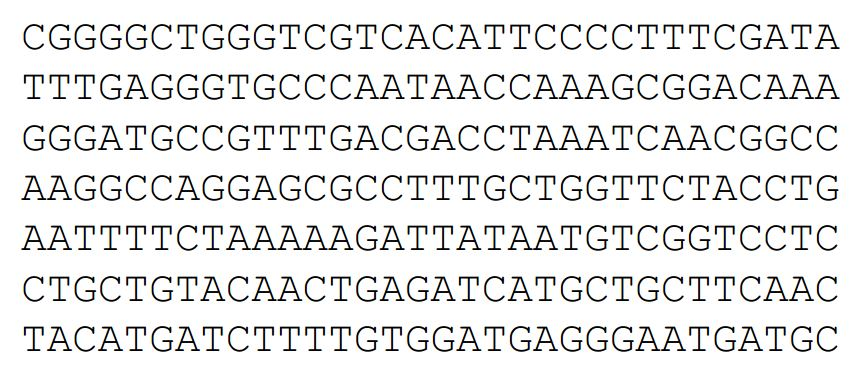
\includegraphics[width=0.6\textwidth]{figures/seq1}
	\caption{Seven random sequences.}
	\label{fig:seq1}
\end{figure}
\begin{figure}[!tb]
	\centering
	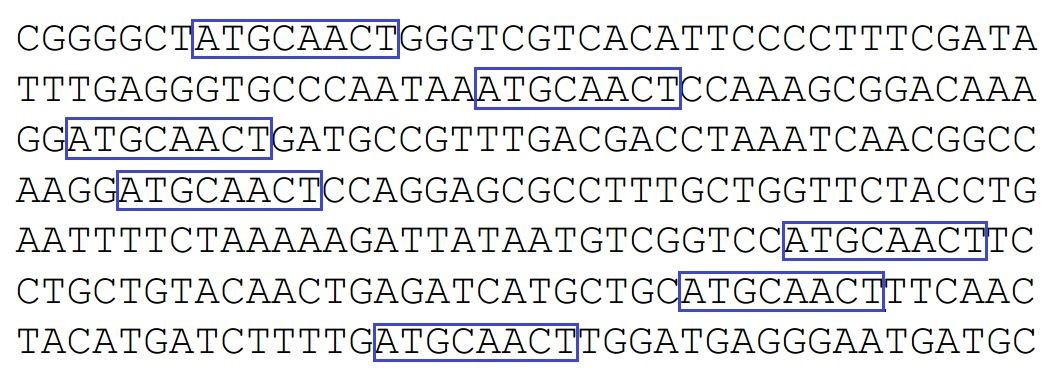
\includegraphics[width=0.75\textwidth]{figures/seq2}
	\caption{The same DNA sequences of \Cref{fig:seq1}
		with the implanted pattern ATGCAACT.}
	\label{fig:seq2}
\end{figure}
\begin{figure}[!tb]
	\centering
	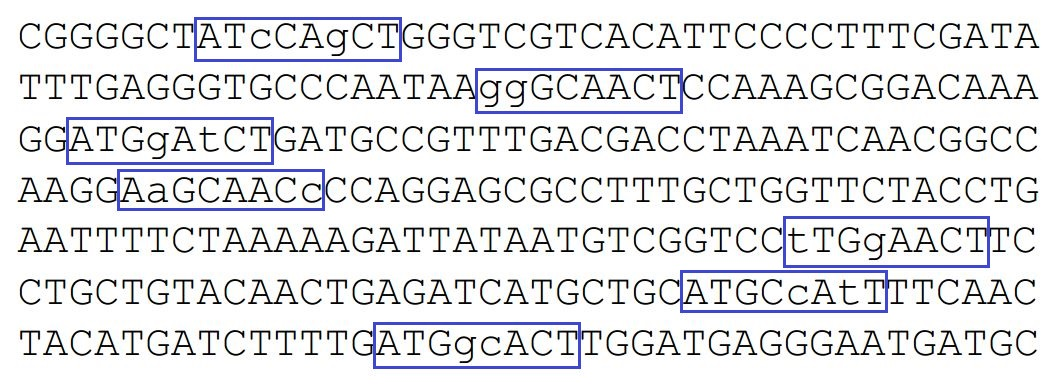
\includegraphics[width=0.75\textwidth]{figures/seq3}
	\caption{Same as \Cref{fig:seq2} with the implanted
		pattern ATGCAACT randomly
		mutated in two positions.}
	\label{fig:seq3}
\end{figure}


\subsection{Alignment Matrix}\index{Alignment Matrix}
To formulate the motif finding problem we first need to define
what we mean by motif. As we saw in \Cref{fig:seq3} there may be
mismatch in some positions of the motifs. Now consider a set of \textit{t} DNA sequences $ S_{1}, S_{2},\ldots, S_{t} $. Each of which has \textit{n} nucleotides. We select one position in each of these \textit{t} sequences, thus forming an array
$ s = (s_{1}, s_{2},\ldots,s_{t}) $, where $ 1 \leq s_{i} \leq n - l + 1$.
Here \textit{l} is the length of the pattern. The superposition
of the \textit{l}-mers of \Cref{fig:seq3} is shown in \Cref{fig:superpose}.
Now taking the \textit{l}-mers starting at these positions
we can compile a \textit{alignment matrix}\index{Alignment Matrix}
of $ t \times l $. The $ (i, j) $th element of the \textit{alignment matrix}
is the nucleotide at the $ s_{i}+j-1 $th position in the
\textit{i}th sequence. Illustrations are shown in \Cref{fig:consensus}.


\begin{figure}%[!tb]
	\centering
	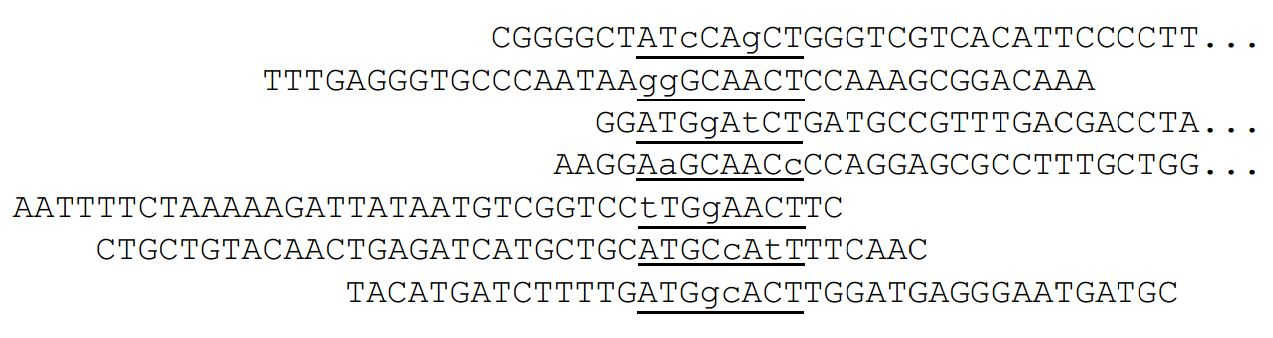
\includegraphics[width=1.0\textwidth]{figures/superpose}
	\caption{Superposition of the seven highlighted 8-mers from \Cref{fig:seq2}.}
	\label{fig:superpose}
\end{figure}




\subsection{Profile Matrix}
The \textit{profile matrix}\index{Profile Matrix} or profile, illustrates
the variability of nucleotide composition at each position for
a particular group of \textit{l}-mers. Let the alphabet $ \Sigma $
in our motif search. Then the size of the \textit{profile matrix} will be
$ | \Sigma | \times l$. For DNA $ | \Sigma | = 4$.  Based on the
\textit{alignment matrix}, we can compute the $ 4 \times l $
\textit{profile matrix} whose $ (i, j) $th element holds the
number of times nucleotide $ i $ appears in column
$ j $ of the \textit{alignment matrix}, where $ i $ varies from 1 to 4.
In \Cref{fig:consensus} we see that positions 3, 7, and
8 are highly conserved, while position 4 is not.

\begin{figure}%[!tb]
	\centering
	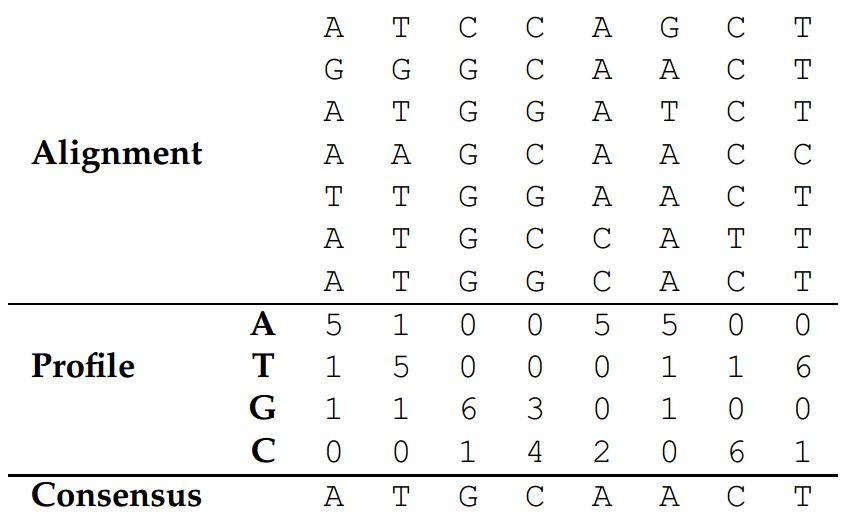
\includegraphics[width=0.7\textwidth]{figures/consensus}
	\caption{The alignment matrix, profile matrix and consensus
		string formed from the 8-mers starting at positions
		$ s = (8, 19, 3, 5, 31, 27, 15) $ in \Cref{fig:seq2}.}
	\label{fig:consensus}
\end{figure}

\subsection{Consensus String}\index{Consensus String}
To further summarize the profile matrix, we can form a consensus string from the most popular element in each column of the alignment matrix. It is the nucleotide with the largest entry in the profile matrix. \Cref{fig:consensus} shows the alignment matrix for s = (8,19,3,5,31,27,15), the corresponding profile matrix, and the resulting
consensus string ATGCAACT.

\subsection{Evaluating Motifs}
By varying the starting positions in $ s $, we can construct a large number of
different profile matrices from a given sample. Some profiles represent high conservation of a pattern while others represent no conservation at all. An imprecise formulation of the Motif Finding problem is to find the starting positions $ s $ corresponding to the most conserved profile. 

\subsubsection{Scoring Function}\index{Scoring Function}
If $ P(s) $ denotes the profile matrix corresponding to starting positions s, then
we will use $ M_{P(s)}(j) $ to denote the largest count in column $ j $ of $ P(s) $. For the profile P(s) in \Cref{fig:consensus}, $ M_{P(s)}(1) = 5, M_{P(s)}(2) = 5$ , and  $ M_{P(s)}(8) = 6 $. Given starting positions s, the consensus score is defined to be $ Score(s, DNA) = \sum_{j=1}^{l}M_{P(s)}(j) $. In our case, $ Score(s, DNA) =
5 + 5 + 6 + 4 + 5 + 5 + 6 + 6 = 42 $. $  Score(s, DNA) $ can be used to measure the strength of a profile corresponding to the starting positions $ s $.

\subsection{Defining The Motif Finding Problem}
the Motif Finding problem can be formulated as selecting starting positions $ s $ from the sample that maximize $ Score(s, DNA) $. 
\begin{table}[H]
	\begin{center}
		\begin{tabular}{p{300 pt}}
			\hline
			\textbf{Motif Finding Problem:}\\
			\textit{Given a set of DNA sequences, find a set of l-mers, one from each
				sequence, that maximizes the consensus score.}\\
			
			\textbf{Input:} A $ t \times n $ matrix of DNA, and l, the length of the pattern
			to find.\\
			
			\textbf{Output:} An array of t starting positions $ s = (s_{1}, s_{2},\dots, s_{t}) $ maximizing \textit{Score(s, DNA)}.\\
			\hline
		\end{tabular}
	\end{center}
\end{table}

\endinput

%\section{What is Bioinformatics}
%Term Bioinformatics was invented by Paulien Hogeweg and Ben Hesper in 1970 as ``the study of informatic processes in biotic systems". Bioinformatics is the application of computer technology to get the information that's stored in certain types of biological data. Bioinformatics provides central, globally accessible databases that enable scientists to submit, search and analyze information. It offers analysis software for data studies and comparisons and provides tools for modeling, visualizing, exploring and interpreting data. Main goal is to convert multitude of complex data into useful information and knowledge.
%
%\subsection{Why Bioinformatics}
%Current biological and medical labs use methods that produce extremely large data sets, which cannot be analyzed by hand - for instance sequencing human genomes. Thus modern biological and medical research and development cannot be done without bioinformatics.
%
%Correctly bioinformatics is being used in following fields:
%\begin{itemize}
%	\item Microbial genome applications
%	\item Molecular medicine
%	\item Gene therapy
%	\item Drug development
%	\item Evolutionary studies
%	\item Biotechnology
%	\item Alternative energy sources
%	\item Crop improvement
%	\item Bio-weapon creation
%	\item Forensic analysis
%	\item Personalized medicine
%	\item Preventative medicine
%	\item Improve nutritional quality
%\end{itemize}
